%!TEX root = ../../../super_main.tex
\subsection{Request Handling}
\label{sub:request_handling}
In the architecture a request from device is going through two different handlers when the server receives it. Firstly it is registered by the NGINX Web Server, which listens on port 8000. Then it will be determined by the webserver which virtual server should handle the request. A virtual server is defined inside the NGINX configuration files, where we for one physical server can specify that it should listen on multiple ports and even have more than one web site listening on the same port, where the requested server name, e.g. www.example.com, determines which of the virtual servers should handle the request. In our case we have two different virtual servers. One for development and one for production. These two virtual servers (server blocks) have been defined in their own configuration file, which then is included by the main configuration file of NGINX. An example of the configuration file for our production site can be seen in \lstref{lst:server_conf}. 

\lstinputlisting[
   caption = {The actual task being executed on a background thread.},
   label = {lst:server_conf},
   float,
]{content/architecture/code_snippets/server.conf}

In line \linesref{lst:server_conf_listen_begin}{lst:server_conf_listen_end} the port that the server should listen on is specified. In our case it would have been ideal to utilize port 80, but the port was already occupied by another server using external IP that was granted to us by the university, instead we were assigned port 8000, which is the one that we utilize as seen in the snippet. This is followed by a directive specifying the root folder of the web site in \lineref{lst:server_conf_root}, and then the index directive specifying that it should prioritize to serve a page called index.php over its HTML counterpart. The server\_name directive was covered by the earlier example, and in this case we are looking at the production server configuration and therefore the names are ``prod.local.element67.dk'' and ``prod.global.element67.dk''. The two location directives as seen in \lineref{lst:server_conf_location} and \lineref{lst:server_conf_location2_begin} specify which page the server should try to serve (relative to the root path) and how it should be done. The syntax for these declarations is the location keyword followed by an optional ``modifier'' and lastly the ``location match'' that the requested URL should match. There are different possibilities for modifiers. In the case of the first location in \lstref{lst:server_conf} we utilize no modifier, meaning that it should be a prefix match. In the case of a prefix match it will try to match the beginning of the given URI (the URL without the hostname in this case) to the location match, and due to the fact that it is a prefix match and the location match is ``/'', all request will be captured by this one, because every URL is prefixed by the root. The second locations modifier is tilde ($\sim$), meaning that the location match will match with a case-sensitive regular expression. The regular expression in the second location match every request with a \mono{.php} suffix in the URI and thereby the directive will capture all requests that is made to a PHP file.
\\\\
When a request is handled by NGINX it will try to find the most specific match, meaning that it will always fall back to the location with the location match of ``/''. Inside this location it will then be checked if it is possible to find a file matching the exact name specified, and if that is not possible we will try to match on folder, and see if that folder contains an index file as specified in the index directive in \lineref{lst:server_conf_index}. If that is not possible the request will internally be redirected to the \mono{index.php} file in the document root, along with any potential query string. This redirection will then be captured by the second location directive in \lineref{lst:server_conf_location2_begin}. This location will as previously mentioned capture all request made to the any PHP files in the system. If any matches the it will choose to use that one, otherwise it will find the index.php file in the root directory and send it this file to the PHP FastCGI Process manager, which runs on a unix socket. An illustration of how a specific request is handled by NGINX is shown in \figref{fig:NGINX_workflow}.

\begin{figure}[!htbp]
    \centering
    \includegraphics[width=0.7\textwidth]{graphic/architecture/NGINX_workflow.pdf}
    \caption{An example of how a request could be handled by NGINX with our configuration.}
    \label{fig:NGINX_workflow}
\end{figure}
\FloatBarrier

Firstly a request is sent to ``prod.local.element67.dk/api/campaigns'', and NGINX will then decide which virtual server should handle the request. In this case it will be the one specified in \lstref{lst:server_conf}, and it will find the best matching location. The request does not have the PHP suffix, so it is captured by the general location. Neither the file or the index file in the directory does in this hypothetical case exist. Therefore the request is internally redirected to ``/index.php'', and is forwarded to the PHP FPM unix socket, where the PHP interpreter and Laravel will take over. 
\\\\
The entry point for the Laravel framework is through the ``index.php'' file that NGINX just redirected to. Here it will will create its own Request object from the request it received from NGINX. This request object is then send to a handler which initiates the flow shown in \figref{fig:laravel_flow}. This flow shows that Laravel utilizes a MVC architecture.

\begin{figure}[!htbp]
    \centering
    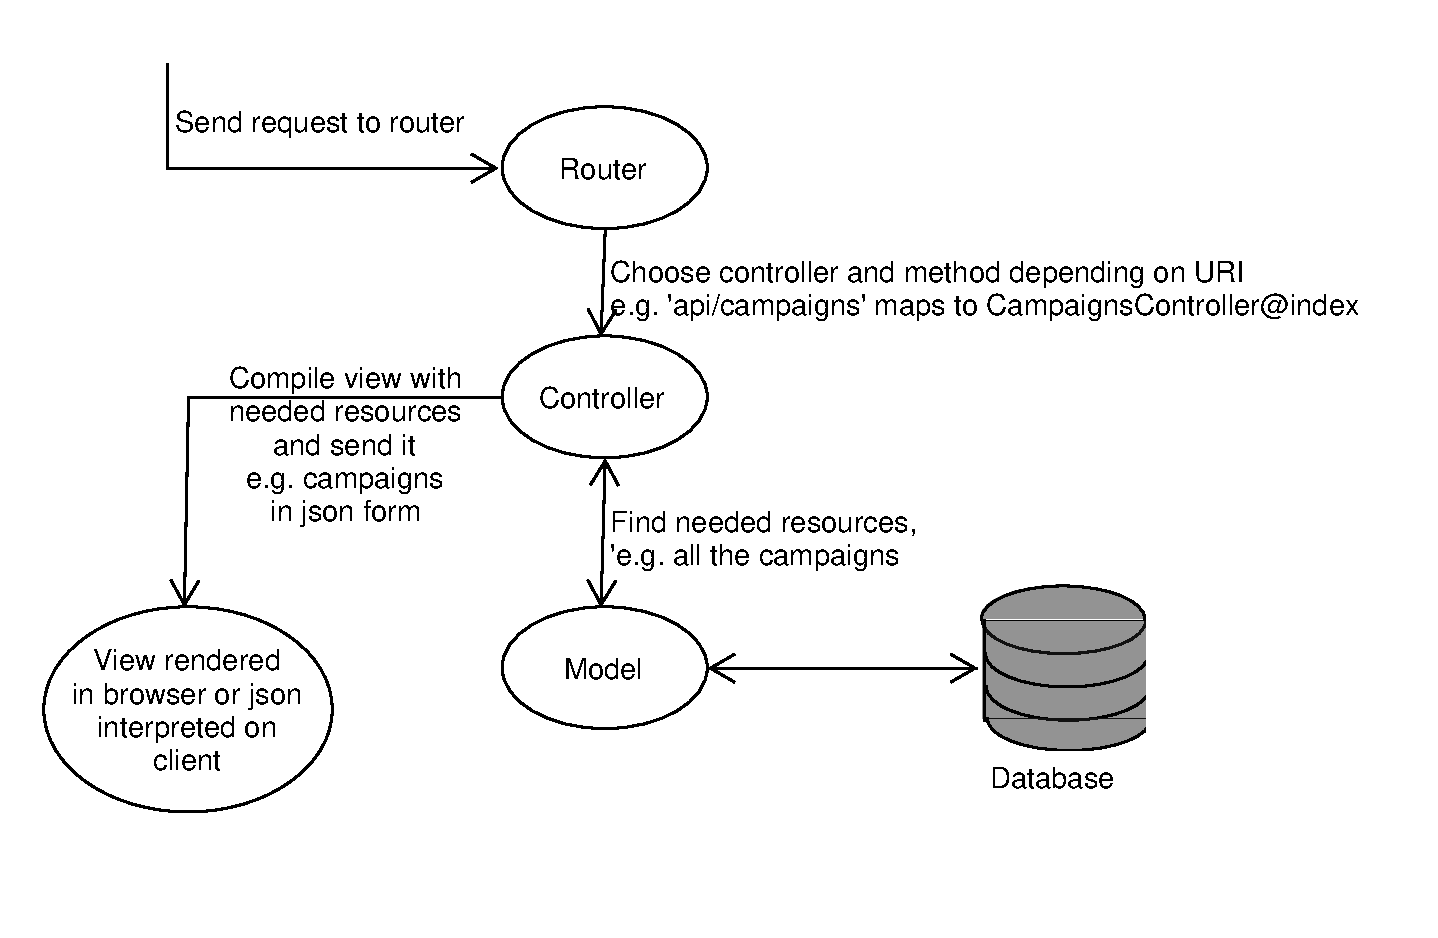
\includegraphics[width=0.7\textwidth]{graphic/architecture/laravel_flow.pdf}
    \caption{An illustration of how a request is traverses through Laravel.}
    \label{fig:laravel_flow}
\end{figure}

Firstly the request is send to the router, which looks at the initial request URI (the URI before NGINX redirected is still available in the HTTP header). Then the router determines which controller-method should be called, retrieves any parameters captured by wildcards in the URI, and invoke the controller-method with these. It is then the controllers job to fetch the needed models to create the requested view, which in the case of an api route will be a JSON response of the given models. The JSON response will then be interpreted by the Android client and the requested information will be shown to the user. 
% https://www.digitalocean.com/community/tutorials/how-to-install-laravel-with-an-nginx-web-server-on-ubuntu-14-04
% https://www.digitalocean.com/community/tutorials/understanding-nginx-server-and-location-block-selection-algorithms
% http://nginx.org/en/docs/http/request_processing.html